\documentclass[11pt]{article}
\usepackage[utf8]{inputenc}
\usepackage{graphicx}
\usepackage[margin = 0.70in]{geometry}
\usepackage{pdfpages}
\usepackage{listings}
\usepackage{xcolor}
\usepackage{array}
\usepackage{appendix}
\usepackage{sectsty}
\usepackage{hyperref}
\usepackage{float}
\usepackage{wrapfig}
\usepackage{subfig}

\definecolor{codegreen}{rgb}{0,0.6,0}
\definecolor{codegray}{rgb}{0.5,0.5,0.5}
\definecolor{codepurple}{rgb}{0.58,0,0.82}
\definecolor{backcolour}{rgb}{0.95,0.95,0.92}

\lstdefinestyle{mystyle}{
    commentstyle=\color{codegreen},
    keywordstyle=\color{blue},
    numberstyle=\tiny\color{codegray},
    stringstyle=\color{codepurple},
    basicstyle=\ttfamily\footnotesize,
    breakatwhitespace=false,         
    breaklines=true,                 
    captionpos=b,                    
    keepspaces=true,                 
    numbers=left,                    
    numbersep=5pt,                  
    showspaces=false,                
    showstringspaces=false,
    showtabs=false,                  
    tabsize=2
}

\lstset{style=mystyle}
\sectionfont{\bfseries\Large\raggedright}
\renewcommand{\thesubsection}{\thesection.\alph{subsection}}
\begin{document}

\begin{titlepage}
    
\begin{center}
    \vspace*{0cm}
    \textsc{\Large DEPARTMENT OF ELECTRONIC AND TELECOMMUNICATION ENGINEERING\\
    [2mm]
    UNIVERSITY OF MORATUWA}\\
    [0.75cm]
    \begin{figure}[htp]
    \centering
    
\includegraphics[width=5cm]{UoMLOGO.png}
    \label{fig:galaxy}
    \end{figure}

    \textsc{\Large EN2550 FUNDAMENTALS OF IMAGE PROCESSING AND MACHINE VISION}\\
    [5mm]
    \line(1,0){300}\\
    [1mm]
    \huge{\bfseries  ASSIGNMENT 02 - Fitting and Alignment} \\
    \line(3,0){300}\\
[1.2cm]  
\end{center}
\begin{center}
    Thanushan K.
    \hspace*{1cm}
    190621M
\end{center}
\vspace*{1cm}
\begin{center}
    This is submitted as a partial fulfilment for the module EN2550.\\
    \line(10,0){50}\\
    [0.5cm]
    \today
    \end{center}
\end{titlepage}

\newpage
\pagenumbering{arabic}
\begin{flushleft}
\vspace*{-1cm}
\hspace*{-3.6cm}
\\
[0.4cm]
\hspace*{-3cm}
\section{RANSAC Implementation}
RANSAC is a general framework used for fitting models when there are outliers present in the images. In this question, we have to fit a circle using the RANSAC algorithm for a randomly generated set of points. The probability that atleast one sample is free from outliers (p) is set to be 0.99. The outlier ratio (e) was set to 0.5, considering the worst case. The threshold of selecting inliers was set to 1. The Samples N was calculated using the following equation.
\begin{equation}\label{Equation 1: Number of samples}
    N = \frac{\log(1-p)}{\log(1-(1-e)^{min_s})}
\end{equation}
Three random samples were selected in each iteration. The circle was found corresponding to the point at each sample. The inliers are found using the threshold. The current set of inliers is compared with the set of inliers obtained from the previous sample and the set with maximum number of inliers is selected. The iteration goes upto N. Then The RANSAC algorithm is run by giving the final set of inliers obtained as the input inorder to obtain the best fit circle. 
\newline
When considering the results, the best fit circle and the circle drawn using the sample points, which give the set with maximum inliers, are almost similar to each other. The code and Output are shown in figure 1 and 2 respectively.    
\begin{figure}[htp]
    \centering
    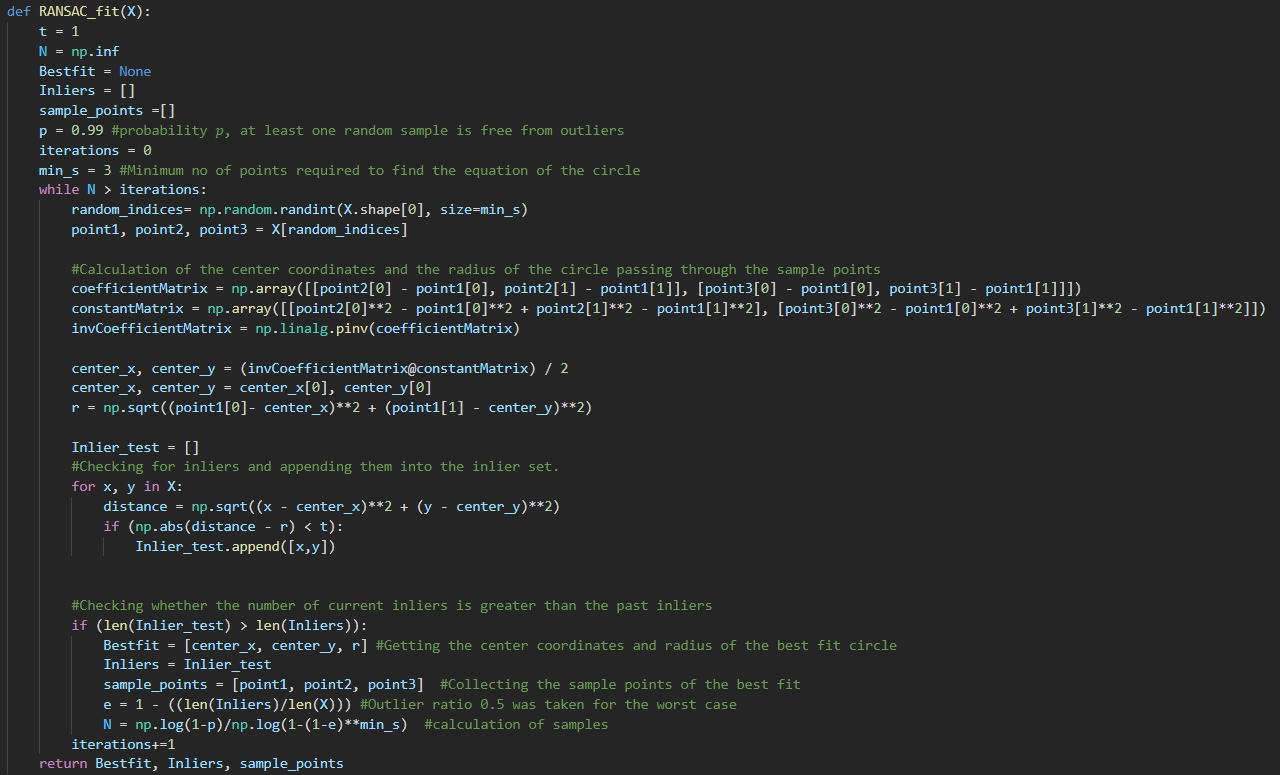
\includegraphics[width=0.7\textwidth]{Question1code.png}
    \caption{Code for RANSAC Algorithm}
\end{figure}
\vspace{-0.5cm}
\begin{figure}[htp]
    \centering
    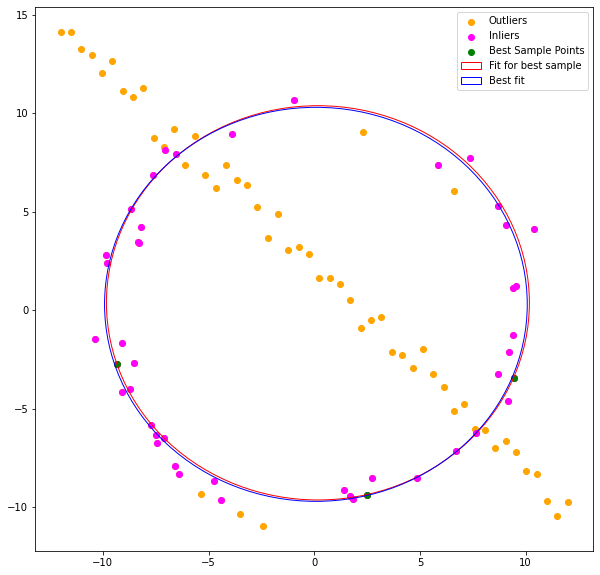
\includegraphics[width=0.5\textwidth]{Question1output.png}
    \caption{RANSAC Circle Fitting}
\end{figure}
\section{Image Warping and Blending by calculating a hormography}
In this question we have to warp and blend one image to another. Initially we have to select 4 points (We get fout points because it is the minimum number of points required to calculate the homography matrix) in the background image and the image to be warped. This can be done by the setMouseCallback function in the opencv library. After getting the four coordinate points of both images, we create a matrix A which is the coeffiecient matrix of the homography vector. We calculate the homography matrix using equation 2. The eigen vector corresponding to the minimum eigen value is taken and constructed into $3X3$ matrix. Then the image is warped according to the corresponing homograpghy matrix and added to the background image.
Two other pairs of images were and the algorithm was tested. The essential codes are shown in figures 3 and 4. The results are shown in figure 5.
\begin{equation}\label{Equation 2: hormography equation}
     A.H = 0
\end{equation}
\begin{figure}
    \centering
    \subfloat[mousePoints function]{{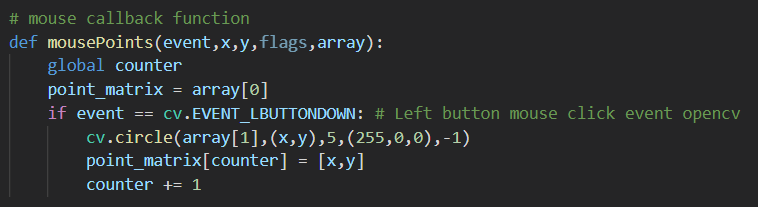
\includegraphics[width=7.0cm]{Question2code1.png}}}
    \qquad
    \subfloat[Loop for selecting points]{{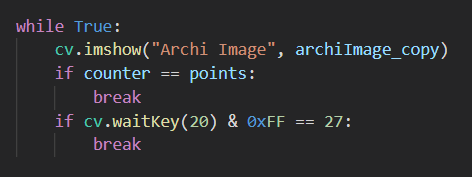
\includegraphics[width=7.0cm]{Question2code2.png}}}
    \caption{Mouse click algorithm}
    \label{fig:example}
\end{figure}

\begin{figure}[htp]
    \centering
    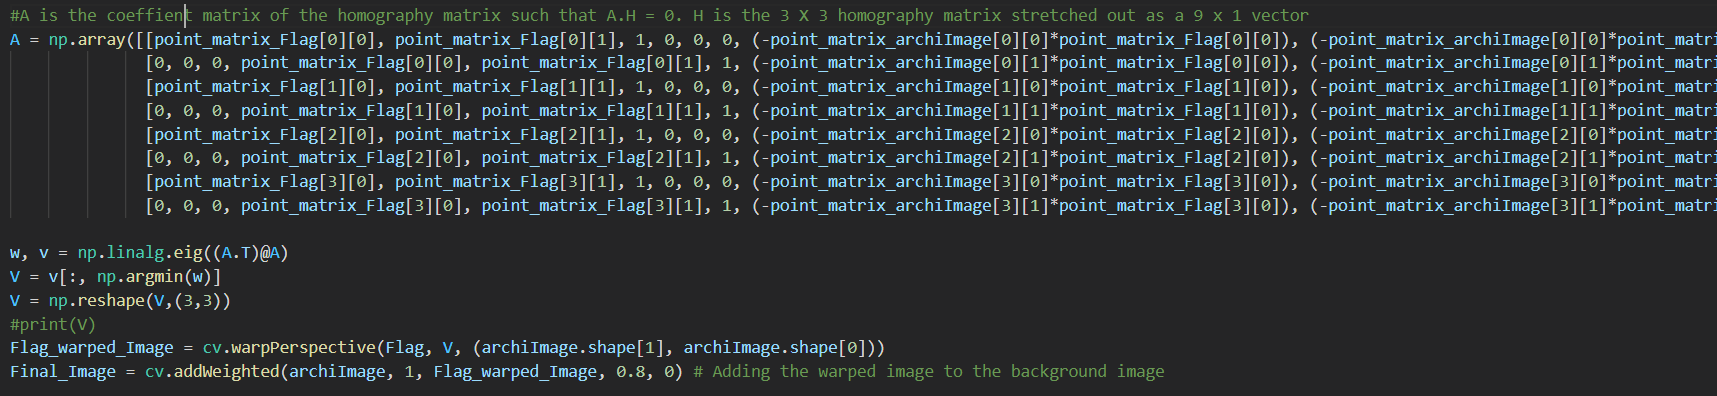
\includegraphics[width=0.75\textwidth]{Question2code3.png}
    \caption{Homography calculation}
\end{figure}

\begin{figure}
    \centering
    \subfloat[Output 1]{{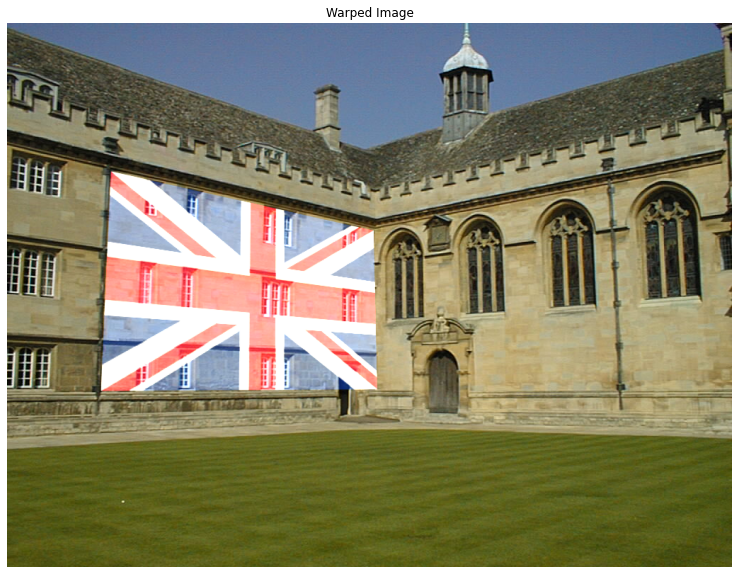
\includegraphics[width=4.0cm]{Question2output21png.png}}}
    \qquad
    \subfloat[Output 2]{{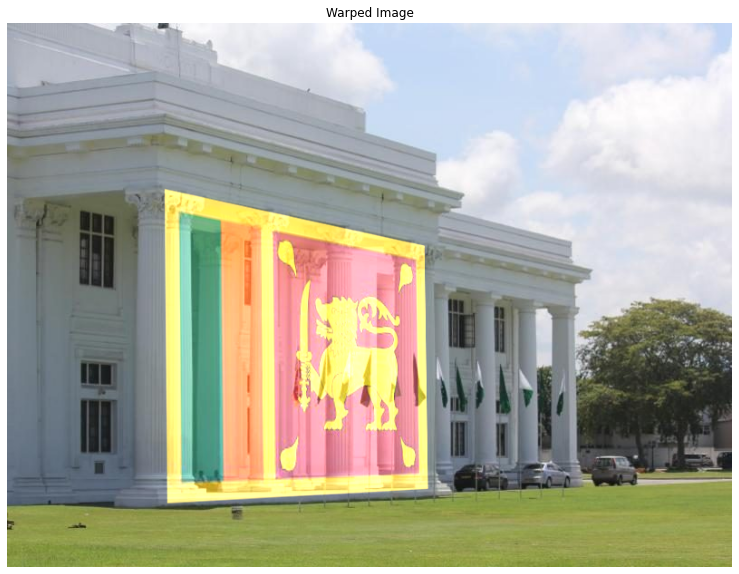
\includegraphics[width=4.0cm]{Question2output2.png}}}
    \qquad
    \subfloat[Output 3]{{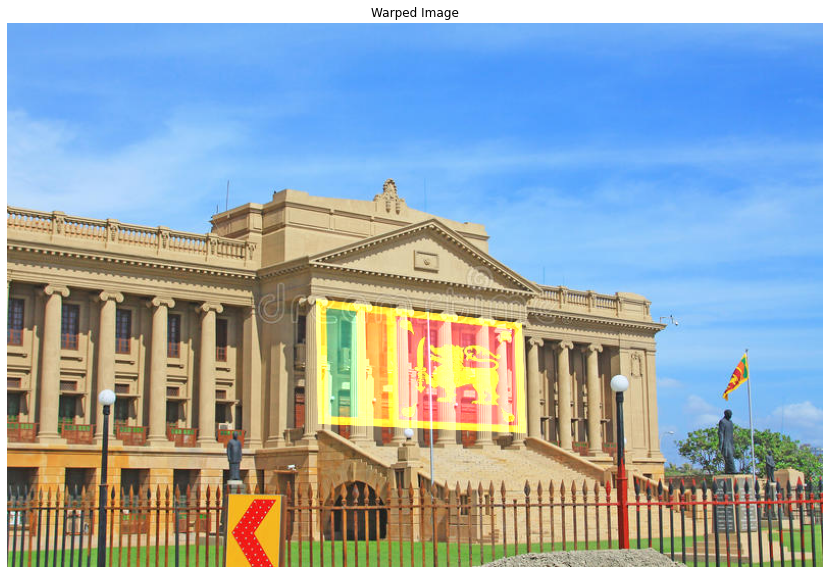
\includegraphics[width=4.0cm]{Question2output3.png}}}
    \caption{Outputs for Warping and blending}
    \label{fig:example2}
\end{figure}






%\hspace{-3cm}
%\begin{figure}[H]
%    \centering
%    \begin{minipage}{.5\textwidth}
%      \centering
%        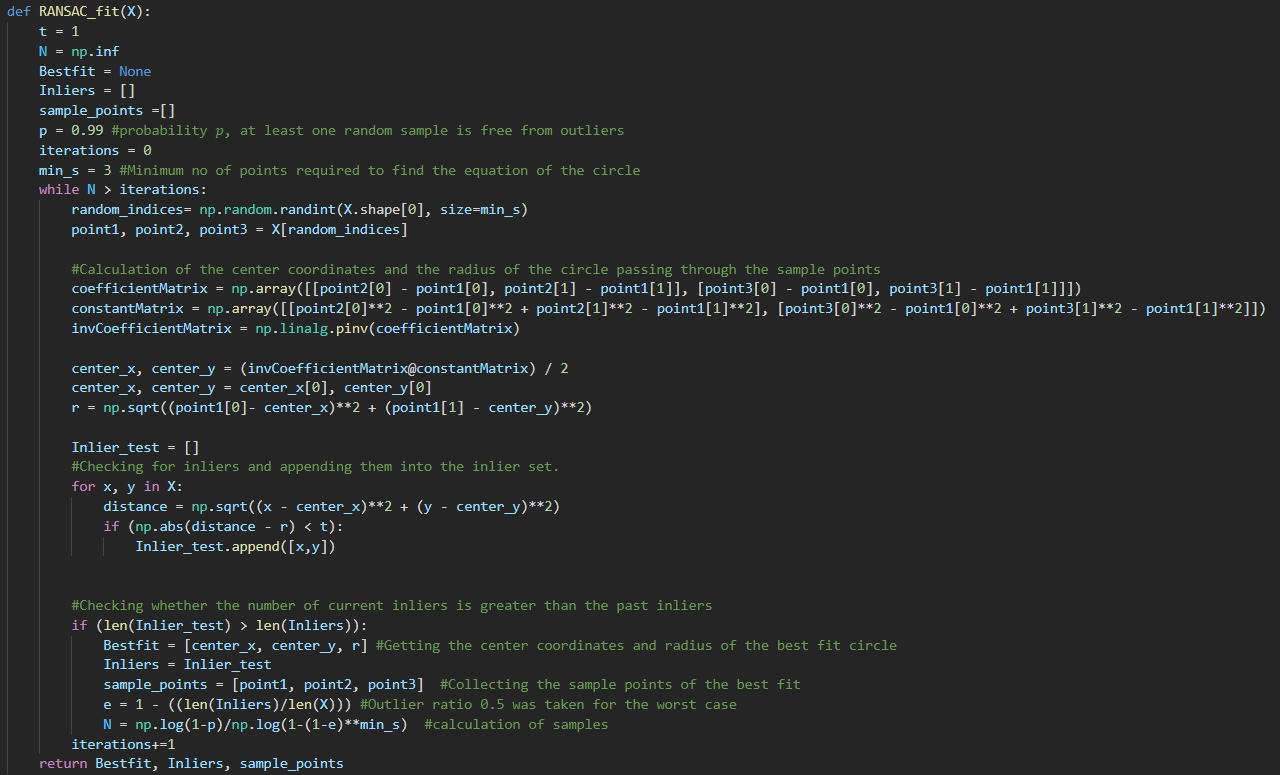
\includegraphics[width=1.\textwidth]{Question1code.png}
%        \caption{label1}
%      \label{fig:test1}
%    \end{minipage}%
%    \begin{minipage}{.5\textwidth}
%     \centering
%        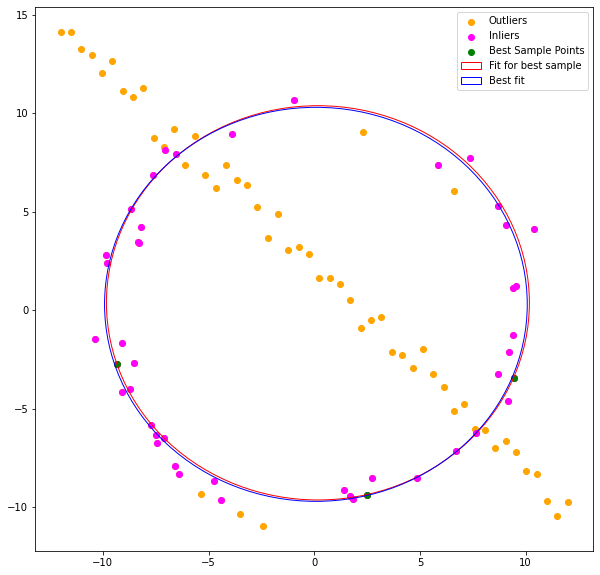
\includegraphics[width=1.\textwidth]{Question1output.png}
%       \caption{label2}
%       \label{fig:test2}
%    \end{minipage}
%\end{figure}


\section{Stitching Two Images by computing a hormography using RANSAC }
Histogram equalization is also an intensity transformation that can be performed in an image such that the pixels are distributed all over the region that the pixels could take values. The result will be an improved version of the image. In this question we have to use a manual function for equalizing the image. Initially, the histogram of the input image is obtained. Then the cdf value is calculated at each point. The calculated cdf value is multiplied by the maximum possible pixel value (L-1) and divided by the product of the dimensions of the input image. The transformation is given by equation 2. 
\begin{equation}\label{Equation 2: Histogram Equalization}
    s_k = \frac{L-1}{MN}\sum_{j=0}^{k} n_j
\end{equation}

\textbf{Code Files} : All relevant codes and files can be found in \href{https://github.com/K-Thanushan/EN2550-Fundamentals-of-Image-Processing-and-Machine-Vision/tree/main/Assignments/Assignment1}{\textbf{\underline{GitHub}}}.

\end{flushleft}

\end{document}